\documentclass[12pt,a4paper]{article}

\usepackage[english,italian]{babel}
\usepackage[T1]{fontenc}
\usepackage[utf8x]{inputenc}
\usepackage{fancyhdr}
\usepackage{indentfirst}
\usepackage{graphicx}
\usepackage{subfigure}
\usepackage{newlfont}
\usepackage{amssymb}
\usepackage{amsmath}
\usepackage{latexsym}
\usepackage{amsthm}
\usepackage{url}
\usepackage{makeidx}
\usepackage[small]{caption}
\usepackage{setspace}
\usepackage{listings}
\usepackage[boxed]{algorithm}
\usepackage{algorithmic}
\usepackage{mathtools}
%\usepackage{authblk}
%\usepackage{apacite}

%\declarepaireddelimiter{\abs}{\lvert}{\rvert}
%\declarepaireddelimiter{\norma}{\lvert}{\rvert}

\floatname{algorithm}{Algoritmo}
\renewcommand{\listalgorithmname}{Elenco degli algoritmi}
\renewcommand{\algorithmicrequire}{\textbf{Input:}}
\renewcommand{\algorithmicensure}{\textbf{Output:}}
\renewcommand{\algorithmicforall}{\textbf{foreach}}
\captionsetup{margin=20pt,font=small,labelfont=bf}
\oddsidemargin=40pt \evensidemargin=25pt
\hyphenation{}
\theoremstyle{plain}              
\newtheorem{teo}{Teorema}[section]
\newtheorem{prop}[teo]{Proposizione}
\newtheorem{cor}[teo]{Corollario}
\newtheorem{lem}[teo]{Lemma}
\theoremstyle{definition}
\newtheorem{defin}{Definizione}[section]
\newtheorem{ese}{Esempio}[section]
\theoremstyle{remark}
\newtheorem{oss}{Osservazione}
%\pagestyle{fancy}\addtolength{\headwidth}{20pt}
%\renewcommand{\chaptermark}[1]{\markboth{\thechapter.\ #1}{}}
%\renewcommand{\sectionmark}[1]{\markright{\thesection \ #1}{}}
%\rhead[\fancyplain{}{\bfseries\leftmark}]{\fancyplain{}{\bfseries\thepage}}
\cfoot{}
%\linespread{1.5}
\newcommand{\df}{\displaystyle\frac}
\newcommand{\seq}[1]{\left<#1\right>}

\title{TableauxProofTool}
\author{	Dott. Fabio Rinnone\\
			Progetto di Logica Computazionale\\
			Corso di Laurea Magistrale in Informatica\\
			Università degli Studi di Catania}
\date{}

\begin{document}

\maketitle

%\tableofcontents

%\begin{abstract}
%\end{abstract}
%\include{qualsiasi_cosa}

\section*{Introduzione}
Lo scopo di questo progetto è stato la realizzazione di un tool, denominato
\emph{TableauxProofTool}, un dimostratore automatico di teoremi della logica proposizionale. Il tool, 
implementato in linguaggio Python \cite{van2007python}, è portabile e quindi eseguibile sulla maggior parte dei sistemi operativi,
tra cui Microsoft Windows e GNU/Linux.

\emph{TableauxProofTool} consente di effettuare le dimostrazioni mediante il metodo classico dei tableaux semantici \cite{fitting1996first}
e mediante le sue più note varianti: i tableaux con merging \cite{d1999tableau}, con lemmi \cite{d1999tableau} e KE \cite{d1994taming}.

L'interfaccia grafica di \emph{TableauxProofTool} è stata realizzata facendo uso del pacchetto PyQT \cite{harwani2011introduction}.

\section*{Sintassi}
Per la rappresentazione delle formule della logica proposizionale è stata introdotta una sintassi specifica: in particolare per la
rappresentazione delle lettere proposizionali è possibile utilizzare le lettere dell'alfabeto ($A, B, C,\ldots$) mentre per la 
rappresentazione dei connettivi logici sono stati utilizzati i seguenti simboli: \texttt{\&} per il connettivo logico \textit{and}, 
\texttt{|} per
il connettivo logico \textit{or} e \texttt{->} per il connettivo logico \textit{implies}.

Un esempio di formula della logica proposizione che è possibile passare in input a \textit{TableauxProofTool} è la seguente:

\begin{displaymath}
\texttt{(p -> (q -> r)) -> ((p | s) -> ((q -> r) | s))}.
\end{displaymath}

\section*{Panoramica di TableauxProofTool}
In \figurename~\ref{fig:figure1} è mostrata la schermata principale del programma. All'avvio dell'applicazione viene mostrato un
framework con un pannello superiore ed uno inferiore. Il pannello superiore presentata una Text Area di input per l'inserimento
delle formule da passare in input, un menu a tendina che permette di selezionare l'algoritmo desiderato e due pulsanti
che consentono rispettivamente di avviare la dimostrazione (Start Proof) o di verificare se la formula sia correttamente 
formattata (Check Formula). Selezionando il pulsante di avvio della dimostrazione viene comunque avviata, prima di eseguire
la dimostrazione, la verifica della corretta formattazione della formula.

Il pannello inferiore contiene una Text Area in cui viene visualizzato il risultato della verifica della formattazione della
formula e i vari passi della dimostrazione.

È possibile caricare una formula precedentemente salvata (formato del file testuale con estensione predefinita 
\texttt{.in}) nonché salvare l'output completo della dimostrazione (estensione predefinita \texttt{.out}).

\begin{figure}[H]
\centering
\linespread{1.0}
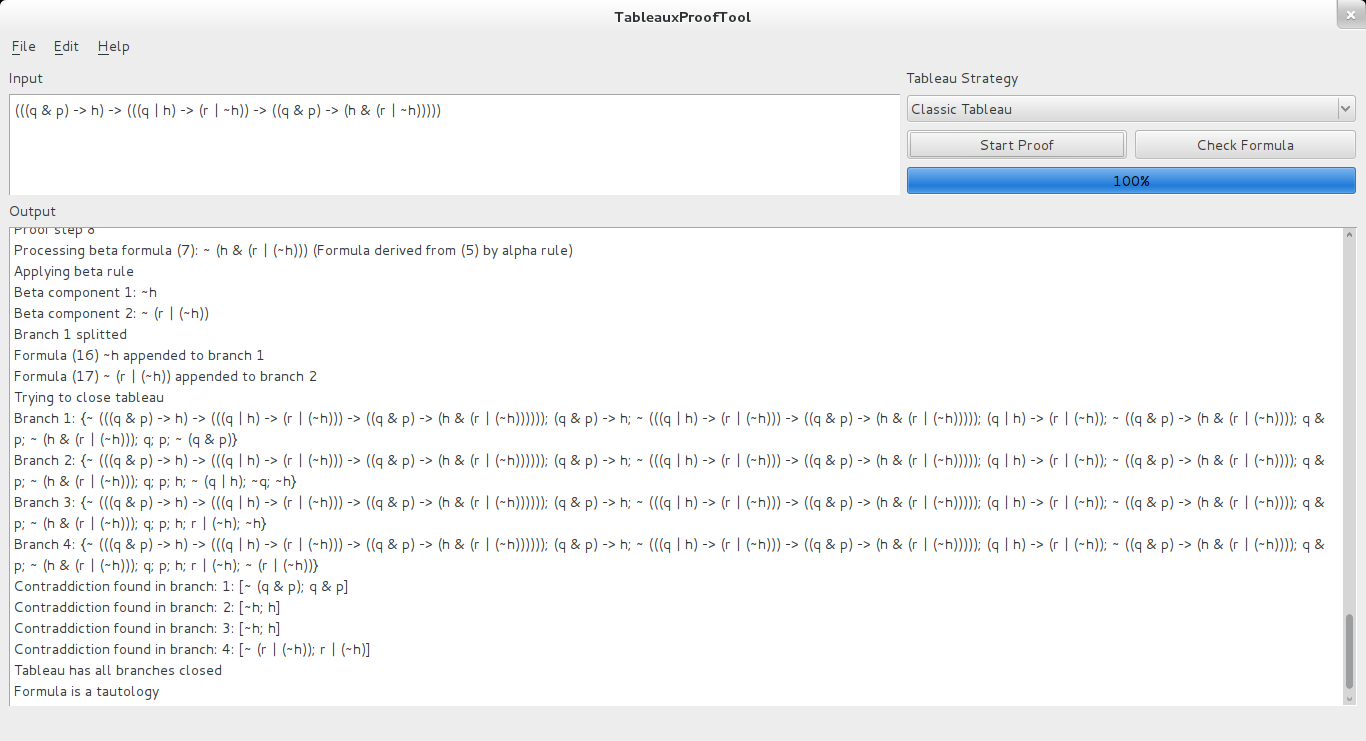
\includegraphics[width=12cm,keepaspectratio]{figures/figure1.eps}
\caption[Schermata principale di Graphtool]{Schermata principale di TableauxProofTool.}
\label{fig:figure1}
\end{figure}

\section*{Implementazione}
Il parsing della formula in input è stato realizzato ricorrendo alle librerie pyparsing \cite{mcguire2007getting} e facendo uso
dell'algoritmo ricorsivo di parsing denominato \emph{packrat} \cite{pyparsingfaq}.

Per rappresentare l'albero della dimostrazione si è optato per l'implementazione classica di un 
albero binario. La struttura dati rappresentate il singolo nodo dell'albero (\texttt{TreeNode}) ha come attributi, un attributo 
denominato \texttt{key}
che memorizza l'indice della formula espansa nell'albero della dimostrazionw, un attributo \texttt{formula} che memorizza la formula espansa
e un attributo \texttt{annotation} che memorizza, per ciascuna formula, un annotazione testuale con informazioni su quale regola
abbia prodotto l'espansione e a il riferimento alle formule dell'albero che l'hanno prodotta.

La struttura dati rappresentante l'albero (\texttt{Tree}) è caratterizzata da due metodi fondamentali per l'implementazione degli algoritmi
di dimostrazione: \texttt{put} e \texttt{split}.

Il primo metodo consente di aggiungere un figlio sinistro al nodo foglia del ramo corrispondente dell'albero e viene richiamato
nel caso in cui viene applicata la $\alpha$-regola o la regola per la doppia negazione nelle implementazioni classica, con lemmi
e merging dei tableaux, ma anche nell'applicazione della $\beta$-regola nel caso specifico dell'implementazione con il metodo KE.

Il secondo metodo consente, invece, di aggiungere due nodi, sinistro e destro, al nodo foglia del ramo corrispondente: in questo
caso il metodo viene richiamato all'applicazione della $\beta$-regola nelle implementazioni classica, con lemmi e merging dei tableaux
e all'applicazione del principio di bivalenza nell'implementazione con il metodo KE.

La classe consente, inoltre, di estrapolare, sotto forma di lista, i rami dell'albero o un ramo specifico a partire dal suo indice.

Le classi che implementano la struttura dati albero e la struttura dati nodo appartengono ad uno specifico package denominato
\texttt{TableauTree}.

Le classi che implementano la dimostrazione, invece, appartengono ad un package denominato \texttt{TableauProof}. La classe principale
astratta del package è la classe \texttt{Tableau} che implementa tutti i metodi comuni a tutti gli algoritmi di dimostrazione
implementati.

\subsection*{Tableaux classici}
La classe che implementa il metodo di dimostrazione classico dei tableaux implementa un attributo di tipo dizionario (Hash Map)
denominato\linebreak\texttt{notAnalysedFormulas}: la chiave corrisponde al numero di ramo dell'albero della dimostrazione, mentre il valore
è una lista di formule non ancora analizzate per il corrispondente ramo. Il metodo principale della classe, denominato
\texttt{proofStep} verifica, per ogni ramo, se sono presenti formule da espandere e, se ne sono presenti, ne estrae una sulla
quale applicare una regola di espansione.

Nella scelta della formula da espandere si è optato per implementare un'euristica che prevede la selezione delle formule in
un ordine specifico: doppie negazioni, $\alpha$-formule e, solo alla fine, $\beta$-formule.

Ad ogni passo di dimostrazione viene richiamato un metodo denominato \texttt{closeTableau} che verifica se, per ogni ramo
sono presenti contraddizioni. Se al termine di ciascun passo il tableaux dovesse risultare chiuso la dimostrazione termina.
Se il tableau non dovesse risultare chiuso si prosegue fino all'esaurimento delle formule da espandere.

Il metodo \texttt{closeTableau} popola un'apposita lista di elementi di tipo booleano che assumono valore \texttt{true} se
il ramo è chiuso, \texttt{false} altrimenti.

\subsection*{Tableaux con merging e con lemmi}
I metodi dei tableaux con merging e con lemmi costituiscono un estensione del metodo di dimostrazione classico. L'implementazione
delle classi è molto simile. A tal proposito è stata progettata una classe astratta, denominata \texttt{ExtendedTableau} che
implementa il metodo che consente di verificare la seguente condizione, a partire da due nodi $n,m$ in due differenti rami:

\begin{equation}
\Delta_n\subseteq \Delta_m.
\label{eq:eq1}
\end{equation}

Le due sottoclassi che implementano rispettivamente i due metodi di dimostrazione, prima dell'applicazione di una regola
di espansione verificano se possibile applicare rispettivamente il merging o il lemma, se verificata la condizione 
\eqref{eq:eq1}. Nel primo caso il ramo può essere marcato come \textit{checked}, nel secondo caso viene appesa la negazione
della formula al ramo corrispondente e il ramo successivamente chiuso.

Nell'implementazione dei tableaux con merging la chiusura viene gestita mediante una lista di booleani analoga a quella
usata nell'implementazione classica ma che tiene conto anche dei rami marcati come \textit{checked}. 

\subsection*{Tableaux KE}
L'implementazione del metodo di dimostrazione KE è realizzata mediante un'apposita classe che estende la classe astratta
\texttt{Tableau}. Il motivo di questa scelta è dettata dal fatto che lo step di dimostrazione è completamente diverso
rispetto ai precedenti metodi. Nella fattispecie sono diverse anche le strutture che gestiscono le formule da espandere
ad ogni passo della dimostrazione.

Sono introdotte due nuove strutture di tipo dizionario: la prima, denominata \texttt{notEAnalysedFormulas} che mantiene
le formule correntemente non E-analizzate per ogni ramo del tableau, la seconda, denominata\linebreak\texttt{notFulfilledBetaFormulas},
che mantiene le $\beta$-formule non trattate.

La procedura \texttt{proofStep} implementa i passi dell'algoritmo descritti in \cite{d1994taming}. È riscritta, rispetto alla
superclasse, la $\beta$-regola ed inoltre è implementata una procedura che gestisce l'applicazione della regola di bivalenza,
denominata \texttt{applyBivalenceRule}.

\subsection*{Diagrammi delle classi}
In Python il tipo \texttt{Formula} riportato nel diagramma delle classi è stato implementato mediante liste annidate, mentre
l'HashMap facendo ricorso ai dizionari.

In figura \figurename~\ref{fig:TableauTree} è riportato il diagramma delle classi relativo al package \texttt{TableauTree},
mentre in figura \figurename~\ref{fig:TableauProof} è riportato il diagramma delle classi relativo al package
\texttt{TableauProof}.

\begin{figure}[H]
\centering
\linespread{1.0}
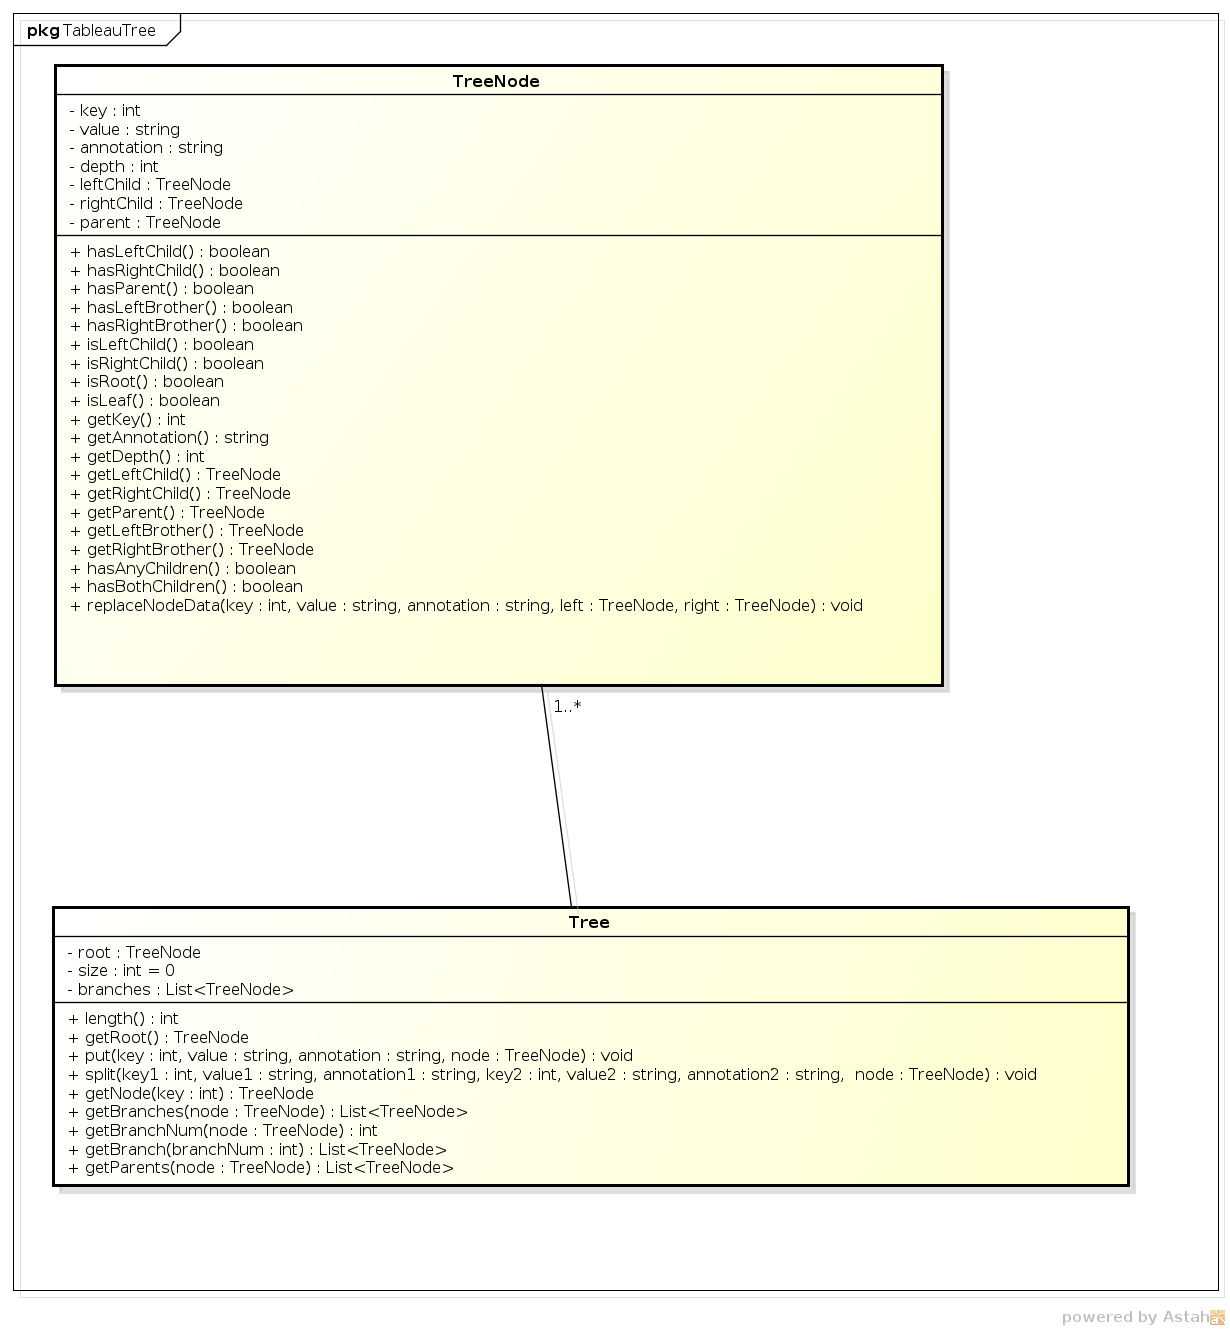
\includegraphics[width=15cm,keepaspectratio]{figures/TableauTree.eps}
\caption[Diagramma delle classi del package TableauTree]{Diagramma delle classi del package TableauTree.}
\label{fig:TableauTree}
\end{figure}

\begin{figure}[H]
\centering
\linespread{1.0}
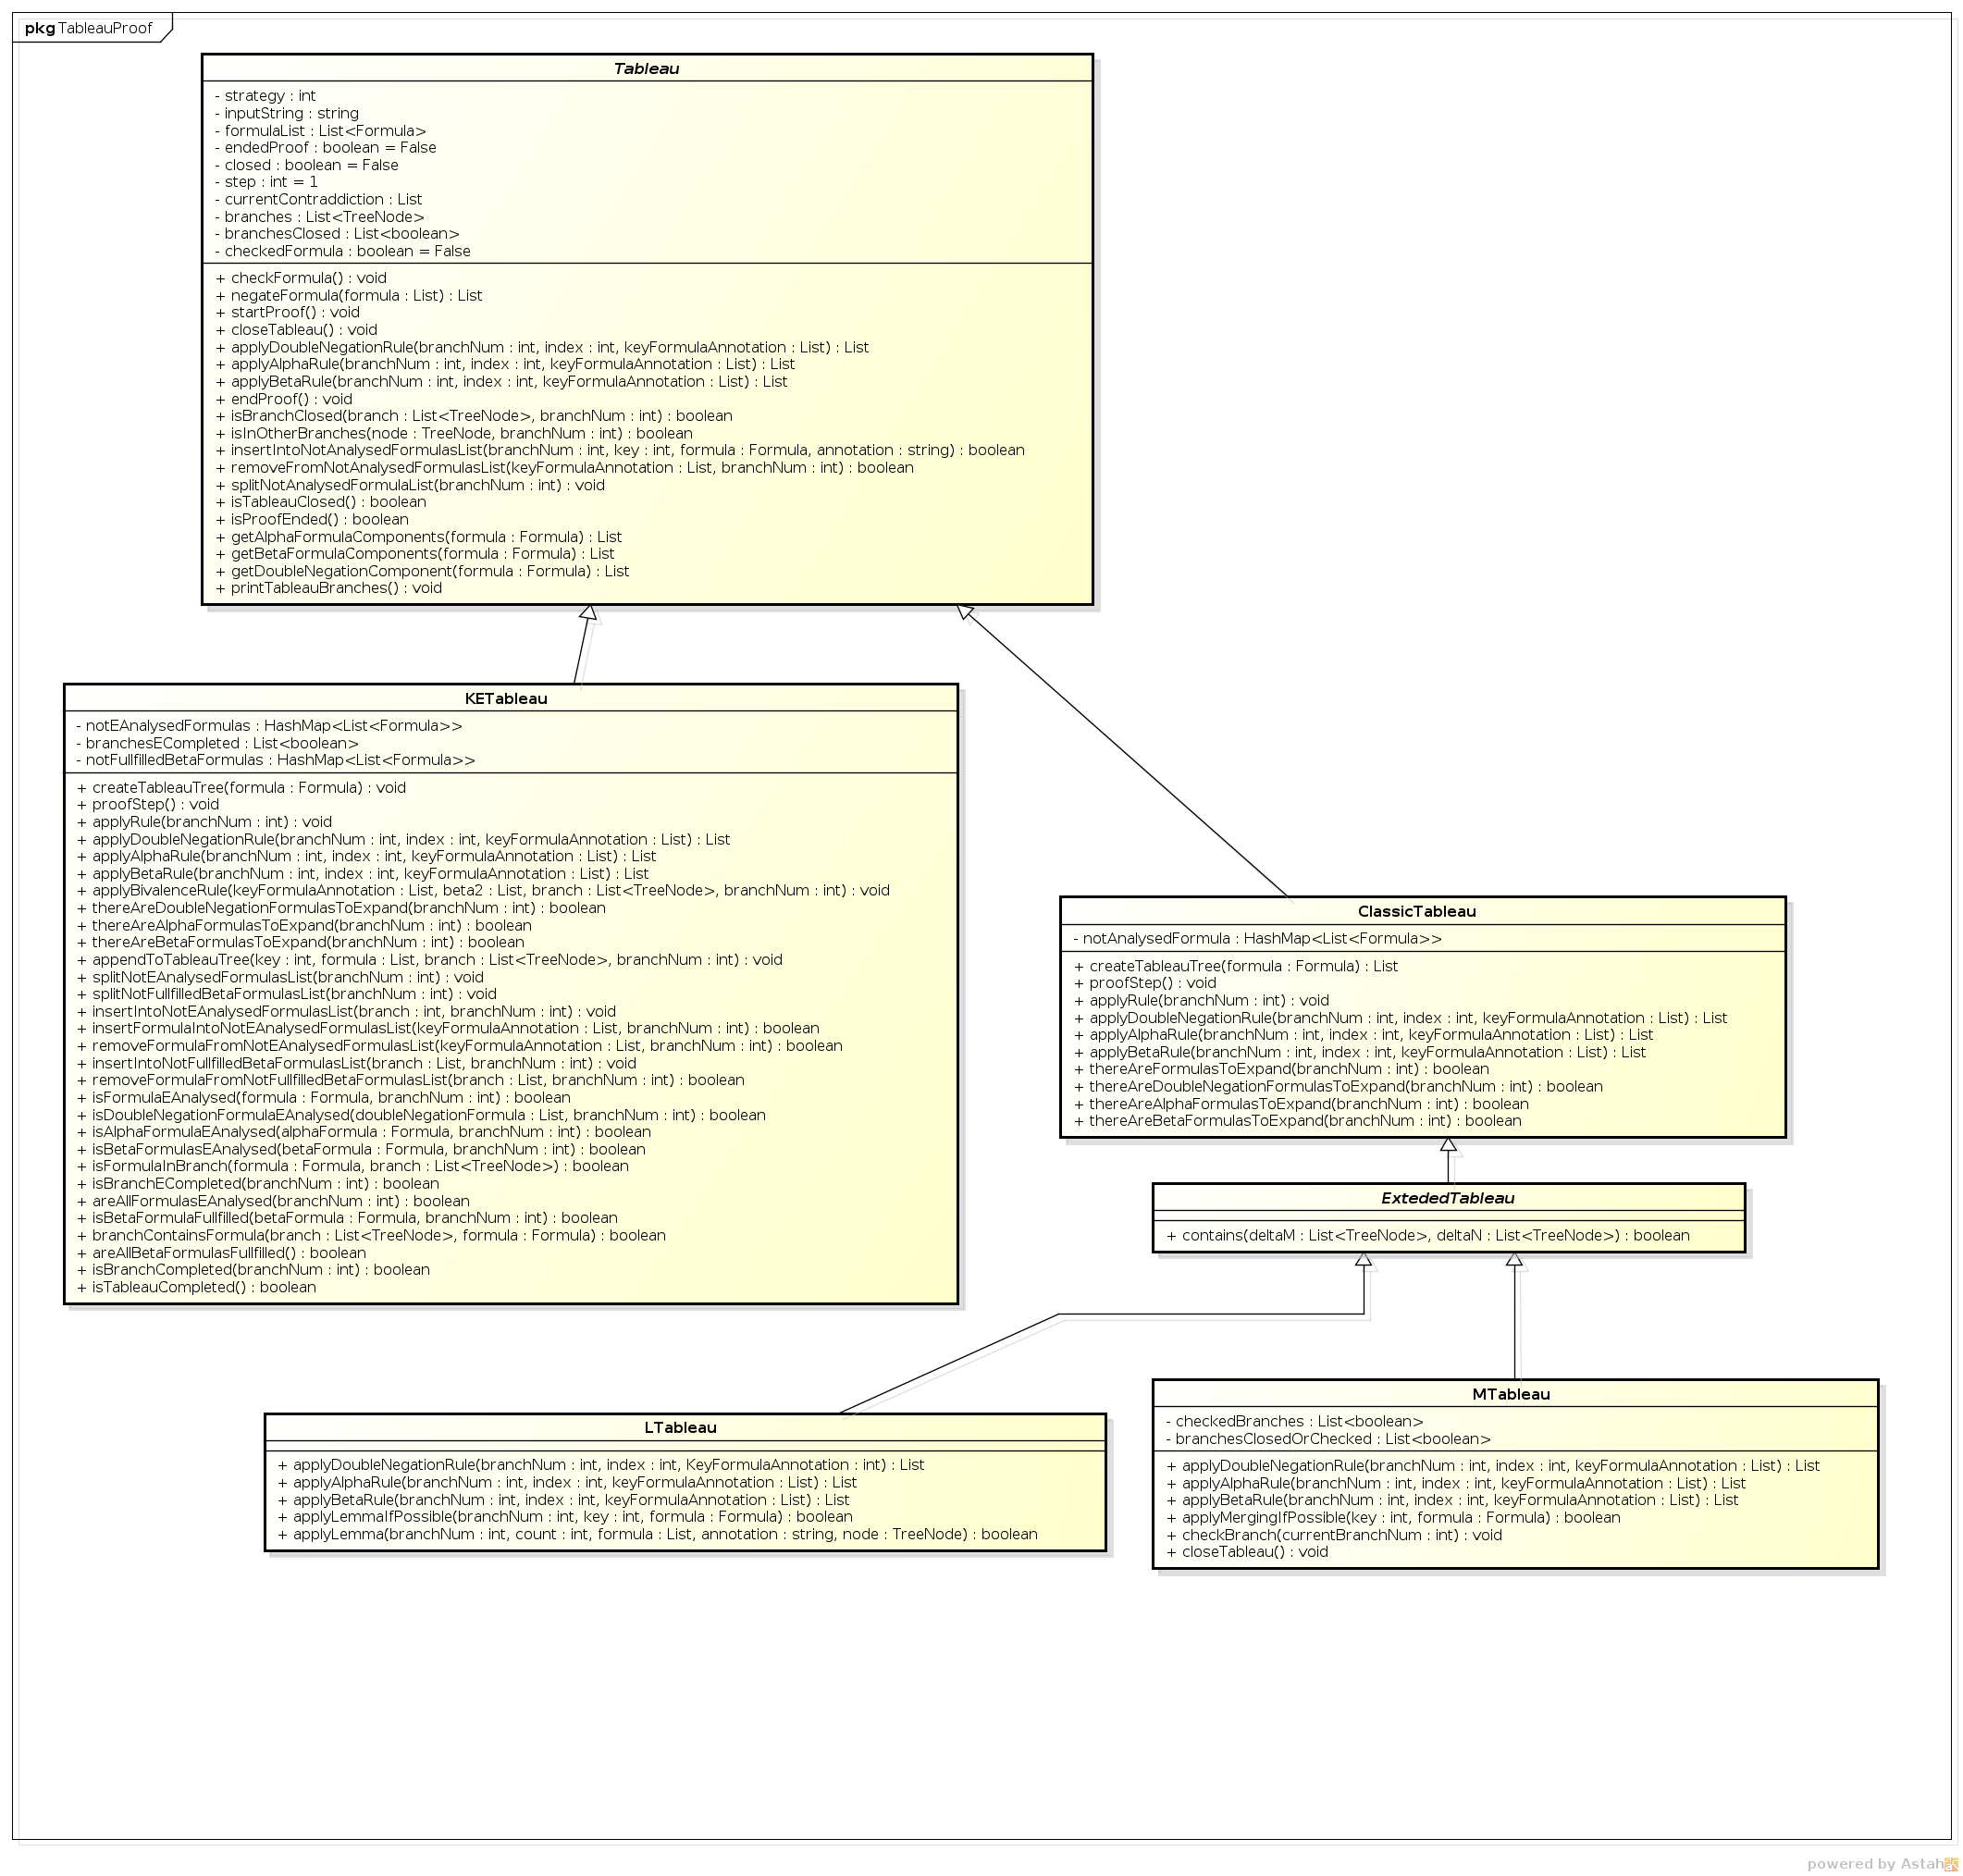
\includegraphics[width=15cm,keepaspectratio]{figures/TableauProof.eps}
\caption[Diagramma delle classi del package TableauProof]{Diagramma delle classi del package TableauProof.}
\label{fig:TableauProof}
\end{figure}

\section*{Risultati}
Il tool è stato testato con diverse formule della logica proposizionale. I risultati ottenuti con la seguente
formula:

\begin{equation}
P\supset (Q\supset R)) \supset ((P\lor S) \supset ((Q\supset R)\lor S))
\label{eq:formula1}
\end{equation} 

sono mostrati in Tabella \ref{tab:tabella1}. In questo caso, data anche la non particolare
complessità della formula, i tempi di esecuzione sono sostanzialmente equivalenti. 

I risultati ottenuti con la seguente formula:

\begin{equation}
(\neg(A\land(B \lor C))\supset (D\supset (F\land (A\land (B\lor C)))))\supset(\neg C\supset (D\supset B))
\label{eq:formula2}
\end{equation}

sono mostrati in Tabella \ref{tab:tabella2}. In questo caso, tuttavia, i tempi di esecuzioni variano sostanzialmente
tra un metodo e l'altro. In particolare il metodo classico risulta più efficiente rispetto agli altri metodi, mentre
il metodo KE, pur ottenendo un'albero con un fattore di ramificazione molto inferiore rispetto agli altri metodi,
risente della maggiore complessità della gestione delle strutture dati che mantengono le formule non E-analizzate
e le $\beta$-formule non trattate, in quanto ad ogni passo dell'esecuzione della dimostrazione, devono essere scandite
le formule di ogni ramo per verificare se tali condizioni risultino o meno verificate.

\begin{table}[H]
\begin{center}
\begin{tabular}{l l}
\hline
Metodo & Tempo esecuzione (sec.) \\
\hline
Tableau classico & 0.00675392150879 \\
Tableau con merging & 0.00838708877563 \\
Tableau con lemmi & 0.0139720439911 \\
Tableau KE & 0.0101838111877 \\
\hline 
\end{tabular}
\end{center}
\caption{Tempi esecuzione Formula \eqref{eq:formula1}.}
\label{tab:tabella1}
\end{table}

\begin{table}[H]
\begin{center}
\begin{tabular}{l l}
\hline
Metodo & Tempo esecuzione (sec.) \\
\hline
Tableau classico & 0.0223960876465 \\
Tableau con merging & 0.0357620716095 \\
Tableau con lemmi & 0.0295519828796 \\
Tableau KE & 0.125766992569 \\
\hline 
\end{tabular}
\end{center}
\caption{Tempi esecuzione Formula \eqref{eq:formula2}.}
\label{tab:tabella2}
\end{table}

\begin{bibliography}{bibliography}
\bibliographystyle{unsrt}
\end{bibliography}

\end{document}
